% Let \( \mathcal{R} = \mathcal{A} \cup \mathcal{B} \) be a set of DPO rewriting rules and let $\mathcal{T}=(T,\mathbb{E},\mathcal{S},w)$ be a weighted type graph over a well-founded commutative semiring such that for every graph $G$ subject to rewriting, we have $\operatorname{Hom}(G,T)\neq \emptyset$. By~\autoref{rem:wf:weight_of_object_geq_1}, for all objects \( G \) subject to rewriting, \(w_\mathcal{T}(G) \succeq_S 1_\mathcal{S} \).
% The rewriting relation \( \Rightarrow_{\mathcal{A},\mathfrak{F}} \) is terminating relative to $\Rightarrow_{\mathcal{B},\mathfrak{F}}$ if (i) for all \(G \Rightarrow_{\mathcal{A},\mathfrak{F}} H\), \( w_\mathcal{T}(G) \succ_S w_\mathcal{T}(H)\), and (ii) for all \(G \Rightarrow_{\mathcal{B},\mathfrak{F}} H\), \( w_\mathcal{T}(G) \succeq_S w_\mathcal{T}(H) \). However, directly verifying all rewriting steps is infeasible due to the potentially infinite number of rewriting steps.

We first introduce the notions of \emph{morphism measurement excluding morphisms in a set}(Definition~\ref{def:weight_excluding_pre}) and \emph{weight of a morphism relative to a morphism-ruler set excluding some specific morphisms}(Definition~\ref{def:weight_excluding}),
to reduce notational overhead (following Endrullis and Overbeek~\cite{endrullis2024generalized_icgt}).
We then recall the notions of traceability of objects (Definition~\ref{def:traceability}) and relative monicity of morphisms (Definition~\ref{def:relative_monicity}),
which are used to define the notion of weighable pushout squares (Definition~\ref{def:weighable}). With the notion of a weighable pushout square, we recall a result from Endrullis and Overbeek~\cite{endrullis2024generalized_icgt} which shows that the weight of the pushout object of a weighable pushout square can be bounded by the weights of the other objects in the pushout square.

\todo{todo to do: pourquoi melange les lettres grecques et latines?}
For any set \( \Gamma \subseteq \operatorname{Hom}(A, G) \),
    we define $\Gamma'$ as the set consisting of all morphisms \( \iota : X \to G \) admitting morphisms \( \zeta \colon X \to A \) and \( \alpha \in \Gamma \) such that $\zeta \star \alpha = \iota$ holds, i.e., such that
     the diagram $\opn{XAG}$ shown below
    %  in Figure~\ref{fig:wf:measurement_of_a_morphism_relative_to_a_morphism_ruler_dfsdfsdsa} 
     is commutative.  Formally,  
    \(
    \Gamma' \overset{\operatorname{def}}{=} \left\{ \iota \in \operatorname{Hom}(X, G)~\middle|~\exists \alpha \in \Gamma,~\exists \zeta:X \to A,~\zeta \star \alpha = \iota \right\}. 
    \)
    % \begin{figure}[H]
    % \centering
    \begin{center}
        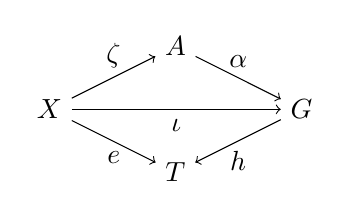
\begin{tikzpicture}[scale=0.8]
            \node (X) at (0,0) {\(X \)};
            \node (A) at (2,1) {\( A \)};
            \node (G) at (4,0) {\( G \)}; 
            \draw[->] (X) -- (A) node[midway, above] {\( \zeta \)};
            \draw[ ->] (X) -- (G) node[midway, below] {\( \iota \)};
            \draw[->] (A) -- (G) node[midway, above] {\( \alpha \)};
            % \node at (2,0.5) {\( = \)};
            \node (T) at (2,-1) {\( T \)};
            \draw[ ->] (X) -- (T) node[midway, below ] {$e$};
            \draw[<-] (T) -- (G) node[midway, below] {$h$};
        \end{tikzpicture}
%     \caption{}
%     \label{fig:wf:measurement_of_a_morphism_relative_to_a_morphism_ruler_dfsdfsdsa}
% \end{figure} 
    \end{center}
    

\begin{definition} 
    \label{def:weight_excluding_pre}
    Let \( \Gamma \subseteq \operatorname{Hom}(A, G) \).
    The \textbf{measurement of a morphism \( h:G \to T \) relative to a morphism-ruler \( e: X \to T \), excluding morphisms in \( \Gamma' \)}, denoted by $m_e(h-\Gamma)$, is defined as:
    \[
        m_e(h-\Gamma) \overset{\operatorname{def}}{=} 
            \card{\set{- \star h = e} \setminus \Gamma'}.
    \]
\end{definition}
\begin{definition}
    \label{def:weight_excluding}
    Let $\mathcal{T}=(T,\mathbb{E},\mathcal{S},w)$ be a weighted type graph. The \textbf{weight of a morphism $h: G \to T$ relative to a set $\mathbb{E}$ of morphism-rulers excluding morphisms in \( \Gamma' \)} is defined as the semiring product of $w(e)^{w_e(h-\Gamma)}$ for $e \in \mathbb{E}$:
    \[ 
        w_\mathcal{T}(h-\Gamma) \overset{\operatorname{def}}{=} \underset{e \in \mathbb{E}}{\bigodot} 
    w(e)^{m_e(h-\Gamma)}.
            \]
\end{definition}
% Consider the pushout square shown below.
% %  in Figure~\ref{fig:preliminaries:pushout_square_traceable_sdldfsfsfsdfkfjsladkj}. Informally, 
%  Any subgraph of the pushout object \(D\) is either the image of \(B\) or the image of \(C\), or is obtained by gluing together parts of the images of \(B\) and \(C\). This intuition is made precise in Definition~\ref{def:traceability}. \todo{todo to do: ????}
% \begin{figure}[H]
%     \centering
%      \resizebox{0.4\textwidth}{!}{
%     \begin{tikzpicture}
%       \node (A) at (0,0) {$A$};
%       \node (B) at (2,0) {$B$}; 
%       \node  (C) at (0,-2) {$C$}; 
%       \node  (D) at (2,-2) {$D$}; 
%       \node  (X) at (4,-2) {$X$};
%       \begin{scope}[nodes=rectangle]          
%       \draw [->] (A) to node [above,label,pos=0.5] {$\alpha$} (B);
%       \draw [->] (A) to node [left,label,pos=0.5] {$\beta$} (C);
%       \draw [->] (B) to node [right,label,pos=0.45] {$\beta'$} (D); 
%       \draw [->] (C) to node [below,label,pos=0.45] {$\alpha'$} (D);
%     %   \draw [->] (X) to node [below,label,pos=0.4] {$h$} (D);
%       \end{scope}
%       \node at ($(A)!.5!(D)$) {$\delta$};
%     \end{tikzpicture}
%     }
%     \caption{}
%     \label{fig:preliminaries:pushout_square_traceable_sdldfsfsfsdfkfjsladkj}
% \end{figure}

\begin{definition}[\cite{endrullis2024generalized_arxiv_v2}]
    \label{def:traceability}
Let $\Delta$ be a class of pushout squares. 
An object $X$ is said to be \textbf{traceable along $\Delta$} if for every diagram $\delta$ in $\Delta$, as shown below:
% in Figure~\ref{fig:preliminaries:pushout_square_traceable_sdlkfjsladkj}, and $h:X \to D$,      
% \begin{figure}[H]
%     \centering
\begin{center}
     \resizebox{0.4\textwidth}{!}{
    \begin{tikzpicture}
      \node (A) at (0,0) {$A$};
      \node (B) at (2,0) {$B$}; 
      \node  (C) at (0,-2) {$C$}; 
      \node  (D) at (2,-2) {$D$}; 
      \node  (X) at (4,-2) {$X$};
      \begin{scope}[nodes=rectangle]          
      \draw [->] (A) to node [above,label,pos=0.5] {$\alpha$} (B);
      \draw [->] (A) to node [left,label,pos=0.5] {$\beta$} (C);
      \draw [->] (B) to node [right,label,pos=0.45] {$\beta'$} (D); 
      \draw [->] (C) to node [below,label,pos=0.45] {$\alpha'$} (D);
      \draw [->] (X) to node [below,label,pos=0.4] {$h$} (D);
      \end{scope}
      \node at ($(A)!.5!(D)$) {$\delta$};
    \end{tikzpicture}
    }
\end{center}
%     \caption{}
%     \label{fig:preliminaries:pushout_square_traceable_sdlkfjsladkj}
% \end{figure} 
  one of the following conditions holds:
    \begin{enumerate}[label=(\alph*)]
        \item\label{traceable:a} there is a morphism $f : X \to B$ such that $h = f \star \beta'$, or
        \item\label{traceable:b} there is a morphism $g : X \to C$ such that $h = g \star \alpha'$.
    \end{enumerate}
    If additionally, 
    whenever \ref{traceable:a} and \ref {traceable:b} hold,
    \begin{enumerate}[label=(\alph*),resume]
        \item 
        there is a morphism $k : X \to A$ such that $h = k \star \alpha \star \beta' $,
    \end{enumerate}
    then we say that $X$ is \textbf{strongly traceable} along $\Delta$.
\end{definition}
Intuitively, in the category \textbf{Graph}, a graph $X$ is $\beta$-strongly traceable along a pushout square, if whenever $X$ occurs in $D$, it occurs either in $B$ or in $C$, and if it occurs in both, then it occurs in $A$ as well.

\begin{remark}[\cite{endrullis2024generalized_arxiv_v2}]
    \label{remark:traceability_graph}
    In \textbf{Graph}, the objects \tikz[baseline=-0.5ex]{
        \node[draw,circle] (x) at (0,0) {};
    } and
    %  \tikz[baseline=-0.5ex]{
    %     \node (x) at (0,0) {$\bullet$};
    %     \node (y) at (1,0) {$\bullet$};
    %     \draw[->] (x) -- (y) node[midway, above] {$x$};
    % } 
    \raisebox{2pt}{
            \scalebox{0.7}{\tikz[baseline=-0.5ex]{
            \node[draw,circle] (x) at (0,0) {};
            \node[draw,circle] (y) at (1,0) {};
            \draw[->] (x)--(y) node[midway, above] {$x$};
        }}}
    (for edge labels $x$) are the only (non-initial) objects that are (strongly) traceable along all pushout squares. 
    Other objects, such as loops~\tikz[baseline=-0.5ex]{
        \node[draw,circle] (x) at (0,0) {};
        \draw[->] (x) edge[loop right]  node[midway, right] {$x$}  (x)
    }, are strongly traceable if all morphisms in the square are monomorphisms.
\end{remark}

\begin{example}
    Consider the following DPO diagram:
    %  shown in Figure~\ref{fig:nwf:two_pushout_squares}.
    \begin{center}
    % \begin{figure}[H]
    %     \centering 
      \resizebox{0.7\textwidth}{!}{
      \begin{tikzpicture}
          \graphbox{\( L \)}{0mm}{-3mm}{34mm}{12mm}{2mm}{2mm}{
              \coordinate (o) at (0mm,-8mm); 
              \node[draw,circle] (l1) at ($(o)+(-10mm,0mm)$) {1};
              \node[draw,circle] (l2) at ($(l1)+(2,0)$) {2};
              \node[draw,circle] (l3) at ($(l1) + (1,0)$) {3};
              \draw[] (l1) -- (l3) node[midway,above] {$a$};
              \draw[] (l3) -- (l2) node[midway,above] {$a$};
          } 
          \graphbox{\( K \)}{40mm}{-3mm}{34mm}{12mm}{2mm}{2mm}{
              \coordinate (o) at (0mm,-8mm); 
              \node[draw,circle] (l1) at ($(o)+(-10mm,0mm)$) {1};
              \node[draw,circle] (l2) at ($(l1)+(2,0)$) {2};
          }  
          \graphbox{\( R \)}{80mm}{-3mm}{45mm}{12mm}{2mm}{2mm}{
              \coordinate (o) at (-5mm,-8mm); 
              \node[draw,circle] (l1) at ($(o)+(-10mm,0mm)$) {1};
              \node[draw,circle] (l2) at ($(l1)+(3,0)$) {2};
              \node[draw,circle] (l3) at ($(l1) + (1,0)$) {4};
              \node[draw,circle] (l4) at ($(l1) + (2,0)$) {5};
              \draw[ ] (l1) -- (l3) node[midway,above] {$a$};
              \draw[ ] (l3) -- (l4) node[midway,above] {$a$};
              \draw[ ] (l4) -- (l2) node[midway,above] {$a$};
          }    
          \graphbox{\( G \)}{0mm}{-22mm}{34mm}{22mm}{2mm}{-3mm}{
              \coordinate (o) at (0mm,-3mm); 
              \node[draw,circle] (l1) at ($(o)+(-10mm,0mm)$) {1};
              \node[draw,circle] (l2) at ($(l1)+(2,0)$) {2};
              \node[draw,circle] (l3) at ($(l1) + (1,0)$) {3};
              \node[draw,circle] (l4) at ($(l2) + (0,-1)$) {6};
              \draw[] (l1) -- (l3) node[midway,above] {$a$};
              \draw[] (l3) -- (l2) node[midway,above] {$a$};
              \draw[ ] (l2) -- (l4) node[midway,right] {$a$};
              \node[draw,circle] (l6) at ($(l1) + (0,-1)$) {7};
              \draw[] (l1) -- (l6) node[midway,left] {$a$};
          }    
          \graphbox{\( C  \)}{40mm}{-22mm}{34mm}{22mm}{2mm}{-3mm}{
              \coordinate (o) at (0mm,-3mm); 
              \node[draw,circle] (l1) at ($(o)+(-10mm,0mm)$) {1};
              \node[draw,circle] (l2) at ($(l1)+(2,0)$) {2};
              \node[draw,circle] (l4) at ($(l2) + (0,-1)$) {6};
              \draw[ ] (l2) -- (l4) node[midway,right] {$a$};
              \node[ draw,circle] (l6) at ($(l1) + (0,-1)$) {7};
              \draw[ ] (l1) -- (l6) node[midway,left] {$a$};
          }    
          \graphbox{\( H \)}{80mm}{-22mm}{45mm}{22mm}{2mm}{-3mm}{
              \coordinate (o) at (-5mm,-3mm); 
              \node[draw,circle] (l1) at ($(o)+(-10mm,0mm)$) {1};
              \node[draw,circle] (l2) at ($(l1)+(3,0)$) {2};
              \node[draw,circle] (l3) at ($(l1) + (1,0)$) {4};
              \node[draw,circle] (l4) at ($(l1) + (2,0)$) {5};
              \node[ draw,circle] (l5) at ($(l2) + (0,-1)$) {6};
              \node[ draw,circle] (l6) at ($(l1) + (0,-1)$) {7};
              \draw[ ] (l1) -- (l6) node[midway,left] {$a$};
              \draw[] (l1) -- (l3) node[midway,above] {$a$};
              \draw[] (l3) -- (l4) node[midway,above] {$a$};
              \draw[ ] (l4) -- (l2) node[midway,above] {$a$};
              \draw[ ] (l2) -- (l5) node[midway,right] {$a$};
          }    
          \node () at (37mm,-8mm) {\( \leftarrowtail \)}; % K -> L
          \node () at (77mm,-8mm) {\( \rightarrowtail \)}; % K -> R
          \node () at (15mm,-18mm) {\( m\ \downarrowtail \)};
          \node () at (37mm,-33mm) {\( \leftarrowtail \)};
          \node () at (58mm,-18mm) {\( u\downarrowtail \)};
          \node () at (102mm,-18mm) {\( \downarrowtail \)};
          \node () at (77mm,-33mm) {\( \rightarrowtail \)}; % C -> H
      \end{tikzpicture}
      }
    \end{center}

   The graph 
   \tikz[baseline=-0.5ex]{
        \node[draw,circle] (x) at (0,0) {};
        \node[draw,circle] (y) at (1,0) {};
        \node[draw,circle] (z) at (2,0) {};
        \draw[->] (x) -- (y) node[midway, above] {$a$};
        \draw[<-] (z) -- (y) node[midway, above] {$a$};
    } is not traceable in both pushout squares. The graph \tikz[baseline=-0.5ex]{
        \node[draw,circle] (x) at (0,0) {};
        \node[draw,circle] (y) at (1,0) {};
        \draw[->] (x) -- (y) node[midway, above] {$a$};
    } is traceable (and strongly traceable) along both pushout squares.
\end{example}

% \begin{example} 
%     Consider the rewriting step shown in Figure~\ref{fig:nwf:rewriting_step_traceability}.
%     The graph \begin{tikzpicture}
%         \node[draw, circle] (x) at (0,0) {};
%         \node[draw, circle] (y) at (1,0) {};
%         \draw[->]  (x) -- (y) node [midway,above] {$c$};
%     \end{tikzpicture} 
%     is traceable along both pushout squares because for every morphism $h$ from this graph to $G$ (resp. to $H$), $h$ factors through $m$ or $l$ (resp. through $u$ or $r$).

%      It is $u$-strongly traceable along the left pushout square, because the only morphism $h:X \to G$ factorizable through $m$ and $l$ has as image the graph \begin{tikzpicture}
%         \node[draw, circle] (x) at (0,0) {z};
%         \node[draw, circle] (y) at (1,0) {y};
%         \draw[->]  (x) -- (y) node [midway,above] {$c$};
%      \end{tikzpicture} and there is a unique morphism $k:X \to A$ such that $h = k \star l \star m$.

%     It is not $u$-strongly traceable along the right pushout square
%     The graph \begin{tikzpicture}
%         \node[draw, circle] (x) at (0,0) {};
%         \node[draw, circle] (y) at (1,0) {};
%         \node[draw, circle] (z) at (2,0) {};
%         \draw[->]  (x) -- (y) node [midway,above] {$c$};
%         \draw[->]  (y) -- (z) node [midway,above] {$c$};
%     \end{tikzpicture} is not traceable along both pushout squares. \todo{todo: why}
% %     because    
% %     \begin{tikzpicture}
% %        \node[draw, circle] (x) at (0,0) {z};
% %        \node[draw, circle] (y) at (1,0) {x};
% %        \node[draw, circle] (z) at (2,0) {y};
% %        \draw[->]  (x) -- (y) node [midway,above] {$c$};
% %        \draw[->]  (y) -- (z) node [midway,above] {$c$};
% %    \end{tikzpicture} is in the pushout object $G$ but in neither $L$ nor $C$.
%    \begin{figure}[H]
%     \centering
%     \resizebox{0.7\textwidth}{!}{
%     \begin{tikzpicture}
%         \graphbox{$L$}{0mm}{0mm}{35mm}{35mm}{2mm}{-7mm}{
%         \node[draw,circle] (1) at (0,0) {x};
%         \node[draw,circle] (2) at (1,-2) {y};
%         \node[draw,circle] (3) at (-1,-2) {z};
%         \draw[->] (1) edge node[midway,right]  {$c$}  node[midway,left]{} (2);
%         \draw[->] (2) edge node[midway,above]  {$c$}  node[midway,below]{}  (3);
%         }
%         \graphbox{$K$}{45mm}{0mm}{35mm}{35mm}{2mm}{-7mm}{
%         % I
%             % \def\x{5};
%             % \def\y{0};
%             \node[draw,circle] (1) at (0,0) {x};
%             \node[draw,circle] (2) at (1,-2) {y};
%             \node[draw,circle] (3) at (-1,-2) {z};
%             \draw[->] (2) edge node[midway,above]  {$c$}  node[midway,below]{}  (3);
%         }
%         \node () at (40mm,-15mm)  {$\overset{l}{\leftarrowtail}$};

%         % \node () at (2.5,-2.5) {$PO$};
%         \graphbox{$R$}{90mm}{0mm}{35mm}{35mm}{2mm}{-7mm}{
%         % R
%             % \def\x{10};
%             % \def\y{-1.1};
%             \node[draw,circle] (1) at (0,-1) {x y z};
%             \draw[->] (1) edge[loop below]  node[midway, below] {$c$}  (1);
%         }
%         \node () at (85mm,-15mm)  {$\overset{r}{\rightarrow}$};

%         \graphbox{$G$}{0mm}{-45mm}{35mm}{35mm}{2mm}{-7mm}{
%         % \node () at (7.5,-2.5) {$PO$};
%         % G
%             % \def\x{0};
%             % \def\y{-5};
%             \node[draw,circle] (1) at (0,0) {x};
%             \node[draw,circle] (2) at (1,-2) {y};
%             \node[draw,circle] (3) at (-1,-2) {z};
%             \draw[->] (1) edge node[midway,right]  {$c$}  node[midway,left]{} (2);
%             \draw[->] (2) edge node[midway,above]  {$c$}  node[midway,below]{}  (3);
%             \draw[->] (3) edge node[midway,above]  {$c$}  node[midway,below]{}  (1);
%         }
%         % C
%         \graphbox{$C$}{45mm}{-45mm}{35mm}{35mm}{2mm}{-7mm}
%         {    
%             \node[draw,circle] (1) at (0,0) {x};
%             \node[draw,circle] (2) at (1,-2) {y};
%             \node[draw,circle] (3) at (-1,-2) {z};
%             % \draw[->] (1) edge node[midway,right]  {$c$}  node[midway,left]{} (2);
%             \draw[->] (3) edge node[midway,above]  {$c$}  node[midway,below]{} (1);
%             \draw[->] (2) edge node[midway,above]  {$c$}  node[midway,below]{} (3);
%             }
%         \node () at (40mm,-55mm)  {$\overset{l'}{\leftarrowtail}$};
%         % H
%         \graphbox{$H$}{90mm}{-45mm}{35mm}{35mm}{2mm}{-7mm}{
%         % R
%             % \def\x{10};
%             % \def\y{-1.1};
%             \node[draw,circle] (1) at (0,-1) {x y z};
%             \draw[->] (1) edge[loop below]  node[midway, below] {} node[midway, below] {$c$} (1);
%             \draw[->] (1) edge[loop above]  node[midway, below] {} node[midway, above] {$c$} (1);
%         }

%         \node () at (85mm,-55mm)  {$\overset{r'}{\rightarrow}$};
%         \node () at (17mm,-40mm) {$m\downarrowtail$};
%         \node () at (62mm,-40mm) {$u\downarrowtail$};
%         \node () at (107mm,-40mm) {$\downarrow m'$};
%     \end{tikzpicture}
%     }
%     \caption{}
%     \label{fig:nwf:rewriting_step_traceability}
%    \end{figure}
% \end{example} 
The following concepts are restricted versions of the concept of monicity.
\begin{definition}[\cite{endrullis2024generalized_arxiv_v2}]
    \label{def:relative_monicity}
    Let $A,B,C$ and $X$ be objects, $\Gamma$ a set of objects, $S$ a set of morphisms to $A$ and $u:C\to A$ a morphism. A morphism $f : A \to B$ is said to be
    \begin{itemize} 
        \item 
            \textbf{monic for $S$} 
            if $g \star f = h \star f$ implies $g = h$ for all $g, h \in S$;
        \item 
            \textbf{$X$-monic} if $f$ is monic for $\operatorname{Hom}(X, A)$;
        \item \textbf{$X$-monic outside of $u$}, if $f$ is monic for \( \operatorname{Hom}(X,A) \setminus \left ( \operatorname{Hom}(X,C) \star u \right ) \);
        \item  \textbf{$\Gamma$-monic} if $f$ is $X$-monic for every $X \in \Gamma$.
    \end{itemize}
\end{definition} 
\begin{example}[Edge-Monicity \cite{endrullis2024generalized_arxiv_v2}]
 
 Let \(f\colon G\to H\) be a morphism in \(\mathbf{Graph}\) that does not identify distinct edges, but may identify distinct nodes. Then \(f\) is not necessarily monic. Indeed, if \(u\neq v\) are nodes of \(G\) with \(f(u)=f(v)\), let \(K\) be the graph consisting of a single node and no edges, and let \(g,h\colon K\to G\) send that node to \(u\) and \(v\), respectively. Then \(g\neq h\) while \(f\circ g=f\circ h\), so \(f\) is not monic.

Nevertheless \(f\) is \(\Gamma\)-monic, where
\[
\Gamma = \left\{ \vcenter{\hbox{
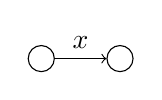
\begin{tikzpicture}[baseline=-0.5ex]
\node[draw,circle] (A) at (0,0) {};
\node[draw,circle] (B) at (1,0) {};
\draw[->] (A) -- (B) node[midway, above] {$x$};
\end{tikzpicture}
}} \mid x \text{ is an edge label} \right\}.
\]
To see this, let \(X\in\Gamma\) and let \(g,h\colon X\to G\) satisfy \(g \star f = h \star f\). Let \(e\) denote the unique edge of \(X\). From \(f(g(e))=f(h(e))\) and the hypothesis that \(f\) is injective on edges we obtain \(g(e)=h(e)\). Since we are working with directed graphs, the images of the two nodes of \(X\) are determined by the image of \(e\), so \(g\) and \(h\) agree on both nodes. Hence \(g=h\), and \(f\) is \(\Gamma\)-monic.

\end{example}
\begin{definition}[\text{\cite[\textdef~4.9]{endrullis2024generalized_arxiv_v2}}]
    \label{def:weighable}
    \ \newline
    \noindent
    \begin{minipage}{0.7\textwidth}
        Let  $\mathcal{T} = (T,\mathbb{E}, S, w)$ be a weighted type graph.
        Consider the pushout square $\delta$ shown on the right. We say that $\delta$ is said to be
         \begin{enumerate}[label=(\alph*)]
        \item \textbf{weighable} with $\mathcal{T}$ if the following hold:
            \begin{enumerate}[label=(\roman*)]
                \item $dom(\mathbb{E})$ is strongly traceable along $\delta$,
                \item $\beta'$ is $dom(\mathbb{E})$-monic,
                \item $\alpha'$ is $dom(\mathbb{E})$-monic outside of $\beta$.
            \end{enumerate}
        \item \textbf{bounded-above} by $\mathcal{T}$ if $dom(\mathbb{E})$ is traceable along $\delta$.
    \end{enumerate}
    \end{minipage}
    \begin{minipage}{0.3\textwidth}
        \begin{center}
            \begin{tikzpicture}[node distance=12mm]
                \node (A) {$A$};
                \node (B) [right of=A] {$B$};
                \node (C) [below of=A] {$C$};
                \node (D) [right of=C] {$D$};
                \draw [->] (A) to node [above, label] {$\alpha$} (B);
                \draw [->] (A) to node [left, label] {$\beta$} (C);
                \draw [->] (B) to node [right, label] {$\beta'$} (D);
                \draw [->] (C) to node [below, label] {$\alpha'$} (D);
                \node [at=($(A)!.5!(D)$)] {$\delta$};
            \end{tikzpicture}
        \end{center}
    \end{minipage}
   
\end{definition}

    Consider the following DPO diagram
    %  shown in Figure~\ref{fig:nwf:dpo_diagram_sdfslafgjsl} 
     that defines a rewriting step \( G \Rightarrow_{\rho,\mathfrak{F}} H \). 
    \begin{center}
        \resizebox{0.3\textwidth}{!}{
        \begin{tikzpicture}
            % [node distance=11mm]
            \node (I) at (0,0) {$K$};
            \node (L) at (-2,0) {$L$};
            \node (R) at (2,0) {$R$};
            \node (G) at (-2,-2) {$G$};
            \node (C) at (0,-2) {$C$};
            \node (H) at (2,-2) {$H$};
            \draw [->] (I) to  node [midway,below] {$l$} (L);
            \draw [->] (I) to  node [midway,below] {$r$} (R);
            \draw [->] (L) to node [midway,right] {$m$} (G);
            \draw [->] (I) to node [midway,right] {$u$} (C);
            \draw [->] (R) to node [midway,left] {$m'$} (H);
            \draw [->] (C) to node [midway,above] {$l'$} (G);
            \draw [->] (C) to node [midway,above] {$r'$} (H);
            \node [at=($(I)!.5!(G)$)] {\normalfont PO};
            \node [at=($(I)!.5!(H)$)] {\normalfont PO};
        \end{tikzpicture}
    } 
    \end{center}
    If the left pushout square is weighable with $\mathcal{T}$ and the right pushout square is bounded above by $\mathcal{T}$, by \cite[Lemma 4.13]{endrullis2024generalized_arxiv_v2}, we obtain:
    \todo{todo to do: rapelle le lemma}

\begin{flalign*}
    w_\mathcal{T}(G) 
        & = \bigoplus_{t_K: K \rightarrow T} 
        \left ( \bigoplus_{\substack{t_C: C \rightarrow T\\ t_K = u \star t_C}}
          w_\mathcal{T}(t_C - u) \right ) 
          \odot
        \left (\bigoplus_{\substack{t_L: L \rightarrow T\\ t_K = l \star t_L}}
        w_\mathcal{T}(t_L) \right )
         \\
    w_\mathcal{T}(H) 
        &  \preceq \bigoplus_{t_K: K \rightarrow T} 
        \left ( \bigoplus_{\substack{t_C: C \rightarrow T\\ t_K = u \star t_C}}
         w_\mathcal{T}(t_C - u) \right ) 
         \odot 
         \left ( \bigoplus_{\substack{t_R: R \rightarrow T\\ t_K = r \star t_R}}
            w_\mathcal{T}(t_R) \right ) \\
\end{flalign*}
According to these results, in \textsection\ref{wf:sec:termination}, we establish a termination criterion by, for every $t_K: K \rightarrow T$, comparing
$\bigoplus_{\substack{t_L: L \rightarrow T\\ t_K = l \star t_L}}
        w_\mathcal{T}(t_L)$ and 
$\bigoplus_{\substack{t_R: R \rightarrow T\\ t_K = r \star t_R}} 
        w_\mathcal{T}(t_R)$.
Before doing so, we introduce the concept of context closure in the following section. 
